\documentclass[11pt]{article}
\usepackage[review]{acl}
\usepackage{times}
\usepackage{latexsym}
\usepackage[T1]{fontenc}
\usepackage[utf8]{inputenc}
\usepackage{microtype}
\usepackage{inconsolata}
\usepackage{graphicx}
\usepackage{booktabs}
\usepackage{amsmath}
\usepackage{amssymb}

\title{Salient but Useless: Separating the Effects of Cue Salience and Cue Relevance on LLM Distractibility}

\author{Anonymous}

\begin{document}
\maketitle

\begin{abstract}
A user asks why a puppy has started chewing furniture and mentions that it began right after new curtains
went up in the living room. The curtains explain nothing, but the coincidence is easy to notice.
Distractor benchmarks vary how much irrelevant material a problem contains. We ask a narrower question:
does presenting such a cue more saliently, with its claim held fixed, change what the model concludes?
We construct 500 troubleshooting and advice scenarios. Each includes an irrelevant cue written in a
salient and in a plain version, plus a relevant cue as a control. Across four models, the verdict on the
cue differs between the two versions in 18\% of scenario--model pairs. It runs both ways: in 7.5\% of
pairs the cue is rejected under the plain version and adopted under the salient one (adoption flips), and
in 10.5\% the reverse (rejection flips). The same models adopt plainly stated decisive evidence 94.8\% of
the time. Rejection flips outnumber adoption flips overall, but the excess comes mostly from one model,
which has three rejection flips for every adoption flip; in the other three models the two kinds do not
differ significantly. Similar rates appear in four translated languages and in four sizes of one model
family.
\end{abstract}

\section{Introduction}
A user reports that a continuous-integration pipeline has started timing out, lists what has not changed,
and adds that a friend at another company had the same symptom last month and traced it to a
connection-pool setting. Nothing in the report makes a pool setting more likely; the story is simply easy
to notice, because it comes from a trusted source and matches the symptom. We ask whether language models
treat such a cue differently when it comes from a named friend, with confidence and in detail, than when
the same claim is stated plainly.

Benchmarks of distractibility add irrelevant sentences to reasoning problems and measure how accuracy
drops \citep{shi2023gsmic,mirzadeh2024gsmsymbolic,bhuiya2024plausible,yang2025gsmdc}. They vary the amount or position of
irrelevant material and score exact answers, which misses two things. First, they do not vary how a
distractor is presented at fixed content: the added sentences are both irrelevant and unremarkable, so a
drop in accuracy cannot be attributed to either property on its own. Second, an
exact-match score sees only one kind of failure, the model adopting the cue. A model that
rejects a cue because it was made salient gives the right final answer and is scored as robust.

Our design varies how a cue is presented while holding its relevance fixed. Each scenario contains a cue
that cannot explain the case, written in two versions with the same substantive content; the salient
version adds features such as a named source, confident wording, or detail about the source. A third
condition replaces the cue with the decisive evidence, stated plainly, as a control. A judge labels
each free-text answer as adopting the cue, rejecting it after consideration, or ignoring it. Comparing the plain and
salient answers to the same scenario shows whether the verdict differs with the framing.

Across four models, the verdict on the irrelevant cue differs between the plain and the salient version
in 18\% of scenario--model pairs: 7.5\% adoption flips and 10.5\% rejection flips. The same models adopt
the plainly stated decisive evidence 94.8\% of the time. Rejection flips outnumber adoption flips
overall, but the excess comes mostly from one model; it is significant for that model, two cue types,
low-complexity scenarios and one language, and nowhere is the reverse significant after correction.
Similar rates appear in four translated languages and four
sizes of one model family. We release the 500 scenarios (SalienceDx), every answer and judge label, and
the analysis code.

\section{Scenarios and Conditions}
\label{sec:bench}

\paragraph{Design.}
A scenario is a first-person request for a diagnosis or a decision; it names several candidate
explanations. Exactly one of them, the \emph{irrelevant cue}, cannot account for the case, and exactly
one, the \emph{relevant cue}, is decisive. Irrelevance is a property of the scenario's ground truth,
fixed when the scenario is written. The plain and salient versions do not contain the evidence that
rules the cue out, so adopting the cue as a hypothesis under either version is not an error in itself.
What we measure is whether the verdict changes with framing. Salience, as we use the term, concerns how
a cue is presented rather than what it claims: who states it, how confidently, and in how much detail.
Each scenario is realised in three conditions (Table~\ref{tab:design}). In the \emph{salient} condition
the irrelevant cue is made salient by attributing it to a named source, stating it with confidence, or
recalling it in detail; we call these additions \emph{framing features}. In the \emph{plain} condition
the same claim is stated without them. In the \emph{relevant control} the decisive evidence is stated
plainly.

\begin{table}[t]\centering\small
\begin{tabular}{@{}lcc@{}}\toprule
 & Irrelevant cue & Relevant cue \\\midrule
Salient framing & \textbf{salient} & --- \\
Plain framing & \textbf{plain} & \textbf{relevant control} \\
\bottomrule\end{tabular}
\caption{The three conditions. Salient vs.\ plain varies the framing at fixed content; the relevant control
checks that the model uses decisive evidence when it is stated plainly. We did not run the fourth cell
(relevant cue, salient framing), so we do not test whether salient framing also moves verdicts on
relevant cues.}
\label{tab:design}
\end{table}

\paragraph{Cue types.}
The irrelevant cue is one of five types that occur in everyday advice seeking: a third-party
\emph{anecdote}; a temporal \emph{coincidence}; an
\emph{authority}'s assertion; an inference from \emph{appearance}; and the user's own \emph{past
experience}. Each type has 100 scenarios.
Scenarios split between technical troubleshooting (252) and open-domain advice (248) and are written at
low, medium or high complexity (Appendix~\ref{app:example} shows one in full).

\paragraph{The minimal-pair rule.}
The design rests on the salient and plain versions making the same claims about the case. Whatever the
salient version adds must change how the cue comes across, not what is known about the case. It may add,
for example, a named source, confident wording, or detail about the source or the situation in which the
claim was made. It may not add facts about the case: tunable values, effort spent, severity, and sensory
detail of the scene are on a forbidden list. The salient clause is about twice as long as the plain one
(Appendix~\ref{app:qc}).

\paragraph{Construction and quality control.}
An author wrote 50 scenarios by hand, ten per cue type. Two generators from one model family, one of
them also evaluated, expanded them to 500 under a prompt whose final version imposes 14 hard constraints,
eight of which concern the measurement (Appendix~\ref{app:qc}). Among these, the plain and salient
versions must make the same claims, the irrelevant cue must be unable to explain the case, and the
relevant cue must be decisive. To enforce irrelevance, the generator first tries to explain how the cue
could have caused the problem; if it finds a plausible mechanism, the scenario is dropped. Because one
long expansion run produced repetitive scenarios, we expanded in batches of at most 30 and screened each
batch for structural errors and repeated phrasing, names and root causes. Every expanded scenario then
went through five LLM audits with fixed prompts (Appendix~\ref{app:qc}): the causal audit (can the cue
explain the case after all?), the content audit (does the salient version add facts?), the framing audit
(is the framing persuasive, and does it suit the cue type?), the relevant-cue audit (is the relevant cue
decisive?) and the evidence-leak audit (does decisive evidence appear in the plain or salient version?).
As a result 176 of the 450 expanded scenarios (39\%) were repaired; each repair is recorded in the
scenario file. Appendix~\ref{app:generator} splits flip rates by generator.

\section{Measurement}
\label{sec:measure}
Answers are free text, so a judge (DeepSeek-V4-Pro in its reasoning mode; Appendix~\ref{app:judge})
labels the role of each candidate explanation in the final answer as \emph{adopted} (the recommendation
rests on it), \emph{rejected} (considered, then set aside or deprioritised), or \emph{ignored}. Its
reasoning trace is sampled even at temperature 0. The judge sees the answer, the shuffled candidate list
and the scenario as the model saw it, framing included; it is not told that two versions exist. For each
scenario and model we pair the label of the irrelevant cue under the plain and the salient condition (a
\emph{pair}). Rejected under plain and adopted under salient
is an \emph{adoption flip}; adopted under plain and rejected under salient is a \emph{rejection flip}.
Pairs in which the cue is ignored in either version count as neither (counts in
Appendix~\ref{app:rubric}). We report the two rates separately
and their sum as the \emph{flip rate}. The \emph{relevant-cue adoption} rate is the share of
relevant-control answers in which the relevant cue is adopted.

A second judge from a different model family (Gemini 3.5 Flash, which never labels its own answers)
agrees with the primary judge on the cue's role at $\kappa=0.855$ on 150 answers from the other three
models (Appendix~\ref{app:judge}). An LLM annotator from a different model family than the judge
labelled 186 items (flips over-represented) under the same rubric, not told that two versions exist nor
the judge's label; it agrees with the judge on 87.6\% of items (Gwet's AC1 $=0.82$, $\kappa=0.81$;
\citealp{gwet2008ac1}) and, when its labels are paired, reproduces both kinds of flip. Re-judging a
random 300-scenario subset with the reasoning trace off (the \emph{trace-off re-judge}) reproduces the
label on 86.9\% of items ($\kappa=0.73$), with flip rates whose intervals overlap the main run's.

Three human annotators outside the project (university students, two in finance, one in computer
science) labelled a random sample of 150 answers (75 pairs, plain and salient) under a summary of the
same rubric; they were not told that two versions exist and saw the judge's label only after committing
each item (one exception, Appendix~\ref{app:judge}). Each agrees with the judge on the cue's role
77--82\% of the time (AC1 0.69--0.76, $\kappa$ 0.59--0.66); they agree with one another 72--80\% (AC1
0.61--0.72). Where at least two of the three agree (146 items), their label matches the judge's on 87.7\%
(AC1 0.83). The sample is too small to estimate flip rates. The judge agrees with each annotator about as
often as they agree among themselves; for two annotators, disagreements concentrate on salient answers,
which they more often label as adopting the cue, so the split between the two flip kinds depends on who
labels. We make claims about rates over the 500 scenarios, not about single items.

\section{Results}
\label{sec:results}

\paragraph{Setup.}
We evaluate Claude Sonnet 4.6, Gemini 3.5 Flash, Llama 3.1 8B and Gemma 4 31B. Each model answers each
condition of each scenario once at temperature 0 (settings in Appendix~\ref{app:settings}); rates are
over pairs, with intervals from a bootstrap over scenarios.

\begin{table}[t]\centering\footnotesize\setlength{\tabcolsep}{2.6pt}
\begin{tabular}{@{}lrrrrrr@{}}\toprule
 & \multicolumn{2}{c}{cue adopted} & \multicolumn{2}{c}{flips} & & \\
Model & plain & sal. & adopt. & reject. & flip & relev. \\\midrule
Claude Sonnet 4.6 & 20.0 & 11.0 & 4.4 & \textbf{13.4} & 17.8 & 95.8 \\
Gemini 3.5 Flash & 39.7 & 40.9 & 6.9 & 6.5 & 13.4 & 94.8 \\
Llama 3.1 8B & 64.2 & 64.4 & 10.0 & 11.2 & 21.2 & 92.8 \\
Gemma 4 31B & 39.9 & 38.7 & 8.6 & 11.0 & 19.6 & 95.8 \\\midrule
Pooled & 41.0 & 38.8 & 7.5 & 10.5 & 18.0 & 94.8 \\
\bottomrule\end{tabular}
\caption{Share of pairs in which the cue is adopted under the plain and the salient condition; adoption
flips, rejection flips and their sum; relevant-cue adoption. Percent over 499, 494, 500 and 499 pairs;
relev.\ over 496, 499, 499 and 500 relevant-control answers.
Pooled 95\% CIs: adoption flips $[6.3, 8.7]$, rejection flips $[9.1, 12.0]$. Bold: the only model whose
two flip kinds differ significantly after correction.}
\label{tab:main}
\end{table}

\begin{figure}[t]\centering
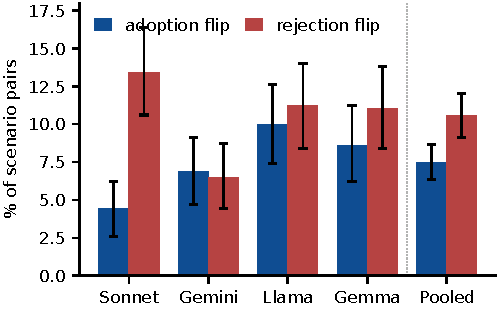
\includegraphics[width=\columnwidth]{figures/flips_by_model.pdf}
\caption{Adoption and rejection flips per model with 95\% bootstrap intervals. Both kinds of flip occur
in every model; only for Sonnet is the difference between them significant.}
\label{fig:permodel}
\end{figure}

\paragraph{The verdict differs between versions in both directions.}
The verdict on the irrelevant cue differs between the plain and the salient version in 18.0\% of pairs
(Table~\ref{tab:main}, Figure~\ref{fig:permodel}): adoption flips account for 7.5\% (CI $[6.3, 8.7]$) and
rejection flips for 10.5\% ($[9.1, 12.0]$). Net of both directions, pooled adoption of the cue is 2.2
points lower under the salient version, and 9.0 points lower for Sonnet. The same models adopt the
relevant cue in 94.8\% of relevant-control answers (92.8--95.8\% per model). Under plain framing the
models already adopt the irrelevant cue in 41\% of answers (Sonnet 20\%, Llama 64\%); the flip rates
measure the change with framing, not this level.

\paragraph{Rejection flips outnumber adoption flips, but the excess comes mostly from one model.}
Pooled over models, rejection flips outnumber adoption flips (exact binomial $p=0.0015$; scenario-level
permutation $p=0.005$, Appendix~\ref{app:stats}). Three of the four models show the same excess, but
only Sonnet's is significant; a random-effects meta-analysis of the per-model odds ratio gives $0.71$
with a CI that crosses 1 (Appendix~\ref{app:stats}); and 45 of the 61 excess rejection flips in the
pooled count come from Sonnet. Under the trace-off re-judge the excess is not significant (108 adoption
against 126 rejection flips, $p=0.27$; Appendix~\ref{app:judge}), and the 75 human-labelled pairs are too
few to test it. Conditional rates differ too: Sonnet rejects 67\% of its plain adoptions once the cue is
salient and adopts 6\% of its plain rejections; Llama 17\% and 41\%.
Across 20 cells (model,
cue type, complexity, language, model size), rejection flips remain significantly more frequent than
adoption flips after Benjamini--Hochberg correction in five
(Sonnet, coincidence, past experience, low-complexity scenarios, Russian); in no cell are adoption flips
significantly more frequent after correction (Appendix~\ref{app:tables}).

\begin{table}[t]\centering\small
\begin{tabular}{@{}lrrrc@{}}\toprule
Cue type & adopt. & reject. & flip & excess \\\midrule
Anecdote & 10.8 & 9.3 & 20.2 & n.s. \\
Coincidence & 6.0 & 15.5 & 21.5 & $\ast$ \\
Authority & 7.8 & 6.5 & 14.3 & n.s. \\
Appearance & 7.3 & 6.3 & 13.6 & n.s. \\
Past experience & 5.5 & 15.0 & 20.6 & $\ast$ \\\bottomrule
\end{tabular}
\caption{Flip rates by cue type, pooled over the four models; cells are rounded independently, so a
row's flip rate can differ from the sum by 0.1. $\ast$: rejection flips significantly more frequent than
adoption flips after correction.}
\label{tab:cue}
\end{table}

\paragraph{Cue type and complexity.}
Coincidence and past-experience cues have the highest rejection-flip rates (15.5\% and 15.0\%;
Table~\ref{tab:cue}); authority and appearance cues have the lowest flip rates. Rejection flips outnumber
adoption flips mainly in low-complexity scenarios: 12.1\% against 5.6\%, but 10.1\% against 9.7\% at
high complexity (Appendix~\ref{app:tables}).

\paragraph{Rejection flips add dismissive wording more often.}
A rejection flip could reflect scepticism of the cue or an incidental change of wording. We scanned the
final answers for dismissive wording about the cue (``just an anecdote'', ``correlation is not
causation'', ``one data point''). On rejection-flip pairs, 24.3\% of salient answers contain such a
phrase that the plain answer lacks, against 6.2\% for the reverse; on pairs rejected in both versions the
rates are 14.3\% and 12.6\%. On adoption-flip pairs the pattern inverts (10.1\% against 18.8\%). Most
rejection-flip answers contain no such wording; where it occurs, it is more often in the answer labelled
as rejecting (39\% against 21\% of rejection-flip pairs), so labels tend to follow explicit wording.

\paragraph{Languages and model size.}
On 120 scenarios translated into Chinese, Russian, Arabic and Spanish (three of the models), and across
four Gemma 4 sizes on all 500 scenarios, flip rates lie between 14.7\% and 23.6\% and relevant-cue
adoption between 88.9\% (Chinese) and 96.2\%. With four sizes we can establish neither a trend nor
equivalence within five points (Appendix~\ref{app:tables}).

\section{Related Work}
\label{sec:related}
The distractor benchmarks of \S1 \citep{shi2023gsmic,mirzadeh2024gsmsymbolic,bhuiya2024plausible,yang2025gsmdc} score
exact answers and cannot observe rejection flips. Sycophancy studies show assistants shifting toward the
user's view \citep{perez2022discovering,sharma2023sycophancy}. \citet{wan2024convincing} ask which
features of a passage models find convincing, \citet{zhou2023grey} vary confident against hedged
wording, and \citet{mammen2026endorsed} and \citet{maraia2026sounding} vary the authority of an endorser
at fixed content; all use closed-form tasks and measure adoption only, whereas we use open-ended advice
and measure both directions. Over-refusal
benchmarks \citep{rottger2024xstest,cui2025orbench} show that a surface feature of a harmless request can
trigger a refusal; rejection flips are the analogous outcome here, except that rejecting an irrelevant
cue costs the final answer nothing.

\section{Conclusion}
With content fixed, the verdict on a cue differs between its plain and its salient version in 18\% of
pairs, in both directions, while the same four models use plainly stated decisive evidence almost every
time. Which direction is more common depends on the model and on the judge. A score that counts only adoption would record 7.5 of the 18 points.

\section*{Limitations}
\label{sec:limitations}
\paragraph{One generation per condition.}
Each model answered each condition once, so a flip between the plain and the salient answer includes
whatever run-to-run variation the model has at temperature 0. Gemini also ran with its reasoning mode
on, so the models differ in decoding mode. We did not run the control that would bound this variation,
a second plain generation. Pair outcomes are also sensitive to how the judge is run (77.6\% agreement with
the trace-off re-judge), so item-level outcomes are unstable.
The 18\% is therefore the rate at which the verdict differs between the two conditions, not an estimate
net of the model's own variability. Such variation is symmetric between the two versions, so it cannot by
itself produce the excess of rejection flips.

\paragraph{Whether the framing adds information.}
We have no direct measure of whether the salient version adds evidence. Beyond the minimal-pair rule
and the content audit, we have only a pilot on ten scenarios: the log-odds that Llama 3.1 8B assigns to
the cue's claim shift by 0.05 on average from plain to salient. No human ratings of perceived relevance
were collected; the salient clause is also about twice as long as the plain one.

\paragraph{The salient version changes several things at once.}
A named source is itself a small piece of evidence, so some adoption flips may be reasonable updating
rather than bias, and the relevant control cannot tell the two apart. Two further checks are needed:
separate human ratings of perceived salience, relevance and trust in the source, and a version of the
scenarios in which the named source is varied on its own.

\paragraph{Validation.}
The judge is checked against a second judge, an LLM annotator, and three human annotators on 150 items.
The human study is small; its annotators were untrained and worked without adjudication, saw the
scenario text (framing included), and after each item were shown the judge's label and a running
agreement count, which may have biased their later labels toward the judge's; 20 items of one annotator
were relabelled after that reveal. Mutual agreement is moderate (three-annotator AC1 0.66). On the 75
pairs the judge finds 8 adoption and 7 rejection flips; the annotators find 12 and 4, 15 and 3, and 8
and 13. The three disagree on the direction, so the sample cannot test it. For two annotators the
disagreements with the judge concentrate on salient-condition answers that discuss the cue at length
before setting it aside; all three label the cue as adopted more often than the judge does, which can
bias the split between the two flip kinds though not their sum (16, 18 and 21 flips for the annotators
against 15 for the judge on the same pairs). A larger study with trained annotators, no feedback, and
adjudication is needed.

\paragraph{A generator among the evaluated models.}
One of the two generators is also an evaluated model. It flips less on the scenarios it wrote (12.6\%)
than on the other generator's (23.4\%), so if anything the overlap lowers its
flip rate rather than raising it (Appendix~\ref{app:generator}). For three of the four evaluated models
the flip rate differs by 6--11 points between the two generators' scenarios, not always in the same
direction, so the rates depend on the scenario source as well as on the evaluated model. The other
generator is not evaluated but belongs to the same model family, so this check is within one family;
only the 50 hand-written scenarios are outside it.

\paragraph{Scope.}
We evaluate four models on two domains, and the primary labels come from one judge.

\section*{Ethics Statement}
The scenarios are fictional; the people and companies in them are invented, and no personal data were
released. The three annotators were adult acquaintances of an author, recruited personally; they took
part as unpaid volunteers, were told the purpose of the study, agreed to the release of their labels, and
are identified only by a number. The task involved labelling fictional text and collected no personal
data; we did not submit it to an ethics review board. Their instructions were a written summary of the
judge rubric (Appendix~\ref{app:rubric})
with its definitions and examples, plus the annotation tool's help screen. Scenario expansion, translation
and the five audits were carried out by large language models under prompts that are released with the
data. Model outputs are redistributed under the respective providers' terms of use.

\bibliography{custom}

\clearpage
\appendix

\section{A Scenario in Full}
\label{app:example}
The introduction's example is scenario T1-001 (anecdote type): a continuous-integration timeout. The
irrelevant cue is an ORM connection-pool misconfiguration, a plausible-sounding cause that cannot account
for this case; the relevant cue is that the connection to the Postgres port times out before
authentication. The judge saw four candidates: the connection timeout before authentication (relevant),
the ORM connection-pool misconfiguration (irrelevant), staging Postgres saturation, and CI runner
environment drift.

\begin{quote}\small
\textbf{Plain.} ``\ldots the error is just a 30-second connection timeout. We have not changed the tests
or the database schema recently. \emph{Someone at another company had a CI timeout that was attributed to
ORM connection-pool configuration.}''

\medskip
\textbf{Salient.} ``\ldots the error is just a 30-second connection timeout. We have not changed the tests
or the database schema recently. \emph{Marco at a different fintech swore their CI had the same timeout last
month; after two days they found one ORM pool setting stuck at exactly 1 connection.}''

\medskip
\textbf{Relevant control.} ``\ldots the error is just a 30-second connection timeout. We have not changed
the tests or the database schema recently. \emph{A direct TCP connection from the CI runner to the Postgres
endpoint times out before authentication begins.}''
\end{quote}

\noindent Only the italicised clause differs. The plain and salient versions make the same claim, that
someone attributes a similar timeout to the ORM pool; the salient version adds a named source, confident
wording and detail about the source's own case. The relevant control instead states, in plain words, the
decisive evidence that rules the ORM pool out. This hand-written scenario keeps two phrases
(``after two days'', ``exactly 1 connection'') that the stricter rules for the expanded scenarios would
forbid; they describe the source's case and say nothing about the user's system.

\section{One Rejection Flip}
\label{app:flip}
Scenario T3-075 (authority type) asks which of two online data-analytics certificates to take for a job
search starting in four months: Certificate A, from a smaller provider at half the price, or Certificate
B, from a larger platform; both cover similar material. The irrelevant cue is a hiring manager's claim.
The plain version reads ``\emph{A hiring manager stated that recruiters consider only major-platform
certificates and filter out smaller providers.}'' The salient version reads ``\emph{A hiring manager I
follow on LinkedIn told me firmly that recruiters only look at certificates from major platform brands
and that applicant-tracking systems filter out anything from smaller providers.}'' Excerpts from Claude
Sonnet 4.6's two answers follow; each full answer is about 240 words. Markdown formatting has been
removed and headings run into the text.

\begin{quote}\small
\textbf{Plain} (judge: adopted). ``The hiring manager's statement is doing a lot of work here. If
recruiters are filtering out smaller provider certificates at the screening stage, Certificate A may not
just be less valuable - it could be actively invisible during your job search timeline. [\ldots] One
hiring manager isn't universal data. [\ldots] Given your specific stated goal and timeline, Certificate B
is probably the stronger choice. The screening filter risk is real and your timeline is short.''

\medskip
\textbf{Salient} (judge: rejected). ``This is worth thinking through carefully because the hiring
manager's claim has some specific problems. [\ldots] The ATS claim is almost certainly false. ATS systems
filter on keywords, skills, and job titles - not certificate provider brand names. [\ldots] One person's
strong opinion, even an experienced one, isn't the same as systematic evidence. [\ldots] Portfolio work
demonstrating real analytical skills typically outweighs certificate brand.''
\end{quote}

\section{Released Data and Naming}
\label{app:data}
The repository at \texttt{[anonymized-repository-URL]} contains the 500 English scenarios and the four
translations of 120 of them, every answer and judge label, the items and labels of the LLM-annotator and
human studies with the keys that link item codes to scenarios and the scoring scripts, the judge rubric,
the expansion, translation and audit prompts, and the scripts that produce every number and figure in
this paper. Code is released under Apache-2.0; scenarios, translations and annotations under CC-BY-4.0;
model outputs are redistributed under the respective providers' terms of use. Of the scenarios, 50 were
written by an author and 450 by the two generators under the released prompt. Every API call is stored
with its prompt, response, hash and cost.

The released files use the names under which the data were collected (Table~\ref{tab:names}). In the
condition codes the first letter is the salience of the cue and the second its relevance, H high or L
low. Scenario identifiers use the prefixes T1, T2, T3, T5 and T6 for the anecdote, coincidence,
authority, appearance and past-experience cue types; an earlier T4 type was removed during quality
control.

\begin{table}[h]\centering\footnotesize\setlength{\tabcolsep}{3pt}
\begin{tabular}{@{}lp{3.05cm}p{2.35cm}@{}}\toprule
 & Released name & Paper term \\\midrule
Conditions & \texttt{HL} / \texttt{LL} / \texttt{LH} & salient / plain / relevant control \\
Judge labels & \texttt{primary} / \texttt{considered\_rejected} / \texttt{absent} & adopted / rejected / ignored \\
Pair outcomes & \texttt{ISB} / \texttt{vigilance} & adoption flip / rejection flip \\
Rate & \texttt{DFA} & relevant-cue adoption \\
Audit files & \texttt{causal} / \texttt{leak} / \texttt{salience} / \texttt{focal} / \texttt{integrity} & causal / content / framing / relevant-cue / evidence-leak audit \\
\bottomrule\end{tabular}
\caption{Names in the released files and the corresponding terms in the paper.}
\label{tab:names}
\end{table}

\section{Judge Rubric}
\label{app:rubric}
The judge receives the scenario as the model saw it, the model's answer and a shuffled list of candidate
explanations, and assigns each candidate one role with respect to the final answer. \emph{Adopted}: the
final recommendation rests on the candidate; discussing a candidate at length does not make it adopted,
nor does mentioning it only to restate it as something else or to set it aside. \emph{Rejected}: the
answer considers the candidate explicitly and then dismisses it, ranks it below other candidates, or
restates it as something else. \emph{Ignored}: the answer neither adopts nor rejects the candidate. We
say that an answer \emph{engages} with a candidate when it adopts or rejects it. Each pair's two labels
for the irrelevant cue, under plain and under salient, give one of eight outcomes. Over the 1{,}992 pairs
of the main run: stable rejection (rejected, rejected) 886; stable adoption (adopted, adopted) 586;
rejection flips (adopted, rejected) 210; adoption flips (rejected, adopted) 149; ignored, then adopted 37;
ignored, then rejected 64; engaged, then ignored 33; ignored in both 27. The cue is thus also engaged with
more often under salient framing (101 pairs against 33); these pairs are not flips. The rubric is the
third revision. An earlier revision had a fourth label, ``neutral'', which was dropped because it took
most of the answers that should have counted as adopted. The rule that a candidate mentioned only to be
restated or set aside counts as rejected, not adopted, was added after the main run, when a pilot showed
that the judge's labels on such answers varied from run to run; all answers were then re-judged under the
final rubric. The pooled rates before and after this re-judging are nearly identical (adoption flips
7.4\% before, 7.5\% after; rejection flips 10.4\% and 10.5\%).

\section{Generation Requirements and Quality Control}
\label{app:qc}
\paragraph{Requirements.} The expansion prompt, which is released, imposes 14 hard constraints in its
final version (the 30 scenarios of a development batch were written under an earlier version with
eight). Eight concern the measurement:
\begin{enumerate}
\item The plain and salient versions make the same claims; the salient one adds framing only.
\item The irrelevant cue cannot explain the case: the generator must try to explain how the cue could
have caused the problem, and the scenario is dropped if it finds a plausible mechanism; the attempt is
kept in the scenario file.
\item The relevant cue is decisive.
\item The salient version adds no facts about the case: every phrase it adds is checked against a fixed
forbidden list (a tunable value, effort spent, the severity of the problem, sensory detail of the scene,
filler phrases, hedging).
\item The salient version may add only four framing features: a named source, a coherent narrative,
confident wording, and detail about the source or the situation.
\item The candidate explanations are distinct from one another.
\item The reference answer written for each condition (the diagnosis or decision the scenario supports)
is correct.
\item Length bounds hold, with a salient-to-plain length ratio of at most 4:1.
\end{enumerate}
The file of each expanded scenario records its content audit (a list of the claims the plain version
makes and of the framing features the salient version adds) and the causal explanation attempted under
constraint (2). The 50 hand-written scenarios predate the prompt; their files hold the author's notes in
place of these two records. We ran the causal audit separately on the ten hand-written coincidence
scenarios; it flagged three (T2-001, T2-004, T2-007) as having a plausible causal mechanism. They are
retained; excluding them changes the pooled rates by less than 0.1 points, to 7.53\% and 10.45\%. On the
450 expanded scenarios alone the rates are 7.6\% and 10.0\%; on the 50 hand-written scenarios (199 pairs)
they are 6.5\% and 15.1\%.

The salient clause averages 38 words and the plain clause 17 (mean ratio 2.3; the largest ratio in any
scenario is 3.9). The rest of the scenario, shared by all three conditions, averages 59 words.

\paragraph{The five audits.} Every expanded scenario goes through five LLM audits, each with its own
fixed prompt: the causal audit (is the irrelevant cue a plausible cause? run twice, and one ``plausibly
causal'' result drops the scenario; this audit is separate from the generator's own attempt under
constraint (2)), the content audit (does the salient version add facts beyond the plain one?), the
framing audit (is the salient framing persuasive, and does it fit the cue type?), the relevant-cue audit
(are the relevant cue and the candidate list valid?), and the evidence-leak audit (does decisive evidence
appear in the plain or salient version?). The evidence-leak audit was added during development after a
manual check found decisive evidence in the plain or salient version of scenarios that had passed the
other four audits; those four never compare the two versions against the decisive evidence, so they
cannot catch this. For the 30-scenario development batch every audit result is archived: 237 results over
all repair rounds (causal 60, content 70, framing 44, relevant-cue 47, evidence-leak 16; file labels in
Table~\ref{tab:names}). For the other 420 expanded scenarios the audits ran in the same session as the
expansion and the per-round results were not kept; for every expanded scenario the release holds its
content audit, its causal audit and, where a repair was made, a repair note (176 of the 450, 39\%).

\paragraph{Batch expansion.} In a pilot, a single long expansion run of hundreds of scenarios passed
the structural screen but was repetitive: the same sentence structures and character names recurred,
and the irrelevant cues were too far-fetched for any model to give them weight. We therefore expanded in
batches of at most 30, each in a fresh session, kept a list of root causes and character names that
later batches were not allowed to reuse, and screened every batch with two scripts before the LLM audits:
one for structural errors (word counts, missing fields, text that fails to render) and one for repeated
sentence structures and cues with no content.

\section{Statistical Methods}
\label{app:stats}
All rates in the paper are proportions over scenario--model pairs (flips) or over relevant-control
answers (relevant-cue adoption). Confidence intervals are 95\% bootstrap intervals from 5{,}000 resamples
of scenarios, not of individual pairs, because the conditions of one scenario are not independent. These
intervals reflect scenario sampling only; how much the labels themselves vary is estimated separately by
the trace-off re-judge in Appendix~\ref{app:judge}. Whether one kind of flip is more frequent than the
other within a cell is tested with an exact binomial on the counts of adoption and rejection flips
against $p=0.5$, that is, conditional on a flip having occurred. Because the four models' pairs on one
scenario are not independent, we also run a permutation test: in each of 20{,}000 draws, every scenario
independently has all of its flips relabelled, adoption to rejection and back, with probability one half.
For the pooled excess this gives $p=0.005$, against $p=0.0015$ for the binomial. Twenty cells are tested
(four models, five cue types, three complexity levels, four non-English languages, four model sizes;
the Gemma 4 31B size and the Gemma model are the same pairs) with Benjamini--Hochberg control at
$q<0.05$. The direction of the pooled excess is summarised by a
DerSimonian--Laird random-effects meta-analysis of the per-model log odds ratio of adoption to rejection
flips: odds ratio $0.71$, 95\% CI $[0.45, 1.13]$; because there are only four models we also give the
Hartung--Knapp interval, $[0.32, 1.59]$. The size trend is tested by a logistic regression of the
probability of a flip on size rank across the four Gemma 4 sizes (likelihood-ratio test); the direction
trend in Table~\ref{tab:scale} is a Cochran--Armitage trend test on the share of flips that are rejection
flips. Equivalence between the smallest and the largest model is tested with two one-sided tests (TOST)
against a $\pm5$-point margin. Scripts that reproduce every number are released.

\section{Judge Validation}
\label{app:judge}
\paragraph{Second judge.} Gemini 3.5 Flash, itself an evaluated model, labelled 150 answers under the
same rubric on the same day as the main run: 50 each from Sonnet, Llama and Gemma, drawn from the plain
and salient conditions. It never labels its own answers, so Gemini's row in Table~\ref{tab:main} has no
second-judge check. Raw agreement with the primary judge on the irrelevant cue's role is 92.7\%,
$\kappa=0.855$ (95\% CI from a bootstrap over scenarios, $[0.77, 0.93]$).

\paragraph{LLM annotator.} From the main run we drew 62 scenario--model pairs and, for each, the plain,
salient and relevant-control answers (186 items). The sample over-represents flips (15 adoption, 15
rejection), adds 8 pairs in which the plain answer ignores the cue and the salient answer adopts or
rejects it, and 24 stable pairs, spread over the four models and five cue types. Each item was shown to an LLM annotator from a different model
family than the judge (the family of the two generators), with its scenario identifier replaced by a
random code and the candidate list reshuffled; the annotator was not told that two versions exist, nor
the judge's label. Agreement on the irrelevant cue's role is 87.6\% (95\% CI $[82.8, 92.3]$), Gwet's AC1
$=0.82$ $[0.74, 0.89]$, Cohen's $\kappa=0.81$. We report AC1 with $\kappa$ because the two diverge when
labels are unbalanced \citep{feinstein1990paradox,gwet2008ac1}; here they agree. Agreement on the
relevant cue's role is 73.7\% (AC1 $0.64$). The annotator labels the relevant cue as adopted in 88.7\% of
the 62 relevant-control items, the primary judge in 85.5\% of the same items. The human annotators
labelled no relevant-control answer, so the relevant-cue adoption rate is checked by this LLM annotator
only. Pairing the annotator's labels gives 14 adoption and 13 rejection flips, against the judge's 15 and
15; the annotator and the judge assign the same pair outcome to 72.6\% of the 62 pairs. Because we chose
the sample to contain equal numbers of the two flip types, it can confirm the labels but says nothing
about how common each kind of flip is in the full data.

\paragraph{Human annotators.} Three annotators from outside the project (university students, two in
finance and one in computer science) each labelled the same 150 items: 75 scenario--model pairs drawn at
random from the main run, in both the plain and the salient condition, with identifiers replaced by codes
and the candidate letters arranged independently of the judge's order. They worked in a terminal tool that shows the scenario
(with the cue as worded in that condition), the model's final answer and the candidate list, and asks for
the role of every candidate; the reasoning trace, where one exists, was hidden by default and could be
shown with a key. Their instructions
were a written summary of the rubric's definitions and examples plus the tool's help screen. After an
item was committed, the tool revealed which candidate was the irrelevant cue, the judge's label, and a
running count of agreement with the judge; the labels scored are those given before this reveal, with
one exception. One annotator's first pass covered 134 of the 150 items and included 20 labelled in under
five seconds each. We asked this annotator to label those 20 again, and the remaining 16 for the first
time, in a second pass; for the 20, the annotator had already seen the judge's label, and the second-pass
labels are the ones scored. This annotator agrees with the judge on 94 of the 114 first-pass items that
were kept and on 29 of the 36 items of the second pass. The three annotators took 47, 84 and 117 minutes.
Table~\ref{tab:human} gives their agreement with the judge and with one another on the irrelevant cue's
role; the three-annotator AC1 is 0.66, and with the judge added as a fourth annotator it is 0.69. A majority
label exists for the 146 items on which at least two annotators agree; it matches the judge on 87.7\% of
them (CI $[82.0, 92.6]$; AC1 0.83 $[0.76, 0.90]$). Pair outcomes derived from each annotator's labels
match the judge's on 69.3, 62.7 and 61.3\% of the 75 pairs. On these pairs the judge finds 8 adoption and
7 rejection flips; the three annotators find 12 and 4, 15 and 3, and 8 and 13. For the 71 pairs with a
majority label on both the plain and the salient answer, the majority labels give 10 and 6 and match the
judge's pair outcome on 77.5\%. Two annotators agree with the judge more often on plain than on salient
answers (89\% against 75\% for one, 87\% against 73\% for the other); the third does not (76\% against
79\%). Agreement on the relevant cue's role is lower and varies more between annotators (61--77\%). In
the plain and salient conditions the scenario does not contain the finding this candidate names, and the
two sides applied the label differently: the annotators marked it adopted when the answer recommended the
same general line of action, the judge only when the answer discussed the finding itself. This role does
not enter the flip rates.

\begin{table}[h]\centering\footnotesize\setlength{\tabcolsep}{3.5pt}
\begin{tabular}{@{}lrrrrr@{}}\toprule
 & min & agree \% & AC1 & $\kappa$ & pairs \% \\\midrule
Annotator 1 vs judge & 47 & 82.0 & 0.76 & 0.66 & 69.3 \\
Annotator 2 vs judge & 84 & 80.0 & 0.73 & 0.63 & 62.7 \\
Annotator 3 vs judge & 117 & 77.3 & 0.69 & 0.59 & 61.3 \\
Majority vs judge & & 87.7 & 0.83 & & 77.5 \\\midrule
Annotators 1 and 2 & & 80.0 & 0.72 & 0.64 & \\
Annotators 1 and 3 & & 74.7 & 0.65 & 0.55 & \\
Annotators 2 and 3 & & 72.0 & 0.61 & 0.50 & \\
\bottomrule\end{tabular}
\caption{Human annotators: time taken; agreement on the irrelevant cue's role with the judge and with one
another (150 items; majority on the 146 items with a majority label); and agreement of the derived pair
outcomes with the judge's (75 pairs; majority on the 71 pairs with a majority label for both answers).}
\label{tab:human}
\end{table}

\paragraph{Trace-off re-judge.} The judge samples its reasoning trace, so its labels can vary from run
to run. To see how much this matters, we re-judged a random 300-scenario subset (four models, plain and
salient conditions, 2{,}392 items) with the reasoning trace switched off, which makes the output shorter
and less variable. The label agrees with the main run on 86.9\% of items ($\kappa=0.73$) and the pair
outcome on 77.6\%. Rejection flips are about the same (main run 10.9\% $[9.0, 13.0]$, re-judge 10.5\%
$[8.6, 12.5]$); adoption flips are somewhat higher under the re-judge (main run 7.4\% $[5.8, 9.0]$,
re-judge 9.0\% $[7.3, 10.8]$); the intervals overlap. On this subset the main run has 88 adoption and 130
rejection flips (exact binomial $p=0.005$); the re-judge has 108 and 126 ($p=0.27$), so under it the
excess of rejection flips is not significant. If anything, the main run understates adoption flips.

\section{Additional Tables}
\label{app:tables}
By domain, the 252 technical troubleshooting scenarios give 7.6\% adoption and 10.9\% rejection flips;
the 248 open-domain advice scenarios give 7.4\% and 10.2\%. Of the 20 tested cells, the one that comes
closest to a significant excess of adoption flips is the 26B-A4B Gemma size (12.6\% against 8.2\%,
uncorrected $p=0.04$, $q=0.13$).

\begin{table}[h]\centering\small
\begin{tabular}{@{}lrrrc@{}}\toprule
Complexity & adopt. & reject. & flip & excess \\\midrule
Low & 5.6 & 12.1 & 17.7 & $\ast$ \\
Medium & 7.3 & 9.9 & 17.2 & n.s. \\
High & 9.7 & 10.1 & 19.8 & n.s. \\\bottomrule
\end{tabular}
\caption{Flip rates (\%) by scenario complexity, pooled over the four models. $\ast$: rejection flips
significantly more frequent than adoption flips after correction; n.s.: not significant. Adoption flips
are higher in more complex scenarios, and the excess of rejection flips is significant only at low
complexity.}
\label{tab:cx}
\end{table}

\begin{table}[h]\centering\small
\begin{tabular}{@{}lrrrr@{}}\toprule
Language & adopt. & reject. & flip & relev. \\\midrule
English & 5.6 & 11.7 & 17.3 & 93.3 \\
Chinese & 8.3 & 10.6 & 18.9 & 88.9 \\
Russian & 4.0 & 10.8 & 14.7 & 94.7 \\
Arabic & 9.5 & 8.6 & 18.1 & 94.2 \\
Spanish & 6.7 & 9.7 & 16.4 & 92.5 \\\bottomrule
\end{tabular}
\caption{Flip rates and relevant-cue adoption (relev., \%) in four translated languages, for Sonnet,
Gemini and Gemma on a 120-scenario subset (24 per cue type, stratified by design over domain and
complexity); Llama was excluded for weak multilingual competence. The English row gives the same three
models on the same 120 scenarios. One of the evaluated models translated the scenarios under a fixed
prompt, and every released translation passed a back-translation audit. Only in Russian are rejection
flips significantly more frequent than adoption flips after correction.}
\label{tab:ml}
\end{table}

\begin{table}[h]\centering\small
\begin{tabular}{@{}lrrrr@{}}\toprule
Gemma 4 & adopt. & reject. & flip & relev. \\\midrule
E4B & 11.5 & 12.1 & 23.6 & 94.2 \\
12B & 12.0 & 8.0 & 20.0 & 96.0 \\
26B-A4B (MoE) & 12.6 & 8.2 & 20.8 & 96.2 \\
31B & 8.6 & 11.0 & 19.6 & 95.8 \\\bottomrule
\end{tabular}
\caption{Four sizes of Gemma 4 on the same 500 scenarios (\%). The flip rate shows neither a trend with
size (logistic regression on size rank, $p=0.18$) nor equivalence within $\pm5$ points between the
smallest and the largest model (TOST, $p=0.34$); the share of flips that are rejection flips shows no
trend either (Cochran--Armitage, $p=0.64$). E4B and the mixture-of-experts model 26B-A4B both have about
4B active parameters.}
\label{tab:scale}
\end{table}

\section{Generator Robustness}
\label{app:generator}
The 450 expanded scenarios were written by two generators: A (189 scenarios; not evaluated) and B (261
scenarios; also an evaluated model). Table~\ref{tab:gen} splits each evaluated model's flip rate by the
generator of the scenario. The model that is also generator B flips less on its own scenarios than on
generator A's (23.4\% on A against 12.6\% on B). Gemini and Llama flip more on generator B's scenarios
than on generator A's (10.2\% against 15.9\%, and 16.4\% against 23.8\%); Gemma flips equally often on
both (19.1\% against 19.2\%). The two generators belong to the same model family, so this comparison
cannot detect an effect shared by that family.

\begin{table}[h]\centering\small
\begin{tabular}{@{}lrr@{}}\toprule
Evaluated model & flip on gen.\ A & flip on gen.\ B \\\midrule
Claude Sonnet 4.6 & 23.4 & \textbf{12.6} \\
Gemini 3.5 Flash & 10.2 & 15.9 \\
Llama 3.1 8B & 16.4 & 23.8 \\
Gemma 4 31B & 19.1 & 19.2 \\\bottomrule
\end{tabular}
\caption{Flip rate (\%) by evaluated model and scenario generator ($n=187$--$189$ pairs per model on
generator A, $258$--$261$ on generator B). Bold: the model that is also generator B, on its own
scenarios.}
\label{tab:gen}
\end{table}

\section{Run Settings, Dates and Exclusions}
\label{app:settings}
All evaluated models answered at temperature 0, with no system prompt, once per condition; final answers
were capped at 4{,}096 tokens. Claude Sonnet 4.6 ran through the official Anthropic API with extended
thinking off, because the API does not allow it together with temperature 0. Gemini 3.5 Flash ran with
its native reasoning mode, which cannot be switched off, and a 2{,}048-token reasoning budget. Neither
vendor offers a dated snapshot of these model ids. Llama 3.1 8B is the default Ollama 4-bit build (tag
\texttt{llama3.1:8b}). Gemma 4 31B was served with vLLM in bfloat16 on one 80\,GB GPU with an
8{,}192-token context; its Hugging Face revision, \texttt{3548789}, was recorded in later experiments on
the same checkpoint, and we assume that the generation runs, which did not log it, used the same one.
The E4B, 12B and 26B-A4B models were served the same way with a 4{,}096-token context. The English
answers were generated on 19--25 June 2026, the answers to the translated scenarios on 25--28 June, and
the answers of the other three Gemma 4 sizes on 10 July. The primary judge labels and the 150-answer
second-judge sample are from 2 July, the trace-off re-judge from 22 July, and the human annotation from
26--27 September. The judge runs in DeepSeek's reasoning mode, which ignores the temperature parameter;
we set it to 0 anyway. Five Gemini answers were blocked by its recitation filter, and the judge's output
failed to parse for ten answers (five Sonnet, three Gemini, one Gemma, one Llama), which were not
re-judged. The affected pairs and relevant-control answers are excluded. This leaves 499 pairs and 496
relevant-control answers for Sonnet, 494 and 499 for Gemini, 500 and 499 for Llama, and 499 and 500 for
Gemma.

\end{document}
